\documentclass[a4paper,french]{article}
\usepackage[utf8]{inputenc}
\usepackage[T1]{fontenc}
\usepackage{babel} 
\usepackage{etex}
\usepackage{fourier}
\usepackage[table]{xcolor}
\usepackage[colorlinks=true,urlcolor=blue]{hyperref}
\usepackage[ant,calculs]{pas-cours}
\usepackage[vmargin=2cm]{geometry}
\usepackage{titlesec}
\usepackage{tcolorbox}
	\tcbuselibrary{skins}
	\tcbuselibrary{theorems}
	\tcbuselibrary{breakable}
\usepackage{cellspace}
\setlength{\cellspacetoplimit}{4pt}
\setlength{\cellspacebottomlimit}{4pt}
\usepackage{tabularx}
\usepackage{lipsum}
\usepackage{multido}
\usepackage{numprint}
\usepackage{dirtree}
\usepackage{listingsutf8}
\usepackage{lipsum}
\lstset{%
	inputencoding=utf8,
	basicstyle=\ttfamily,%
	numbers=left, 
	numberstyle=\color{red!50!yellow}\tiny, 
	stepnumber=1, 
	numbersep=5pt, 
	language=[LaTeX]TeX, 
	backgroundcolor=\color{black},
	frame=shadowbox,
	rulesepcolor=\color{gray!80},
	rulecolor=\color{black},
	framexleftmargin=10pt,
  columns=flexible,
  keepspaces=true,
  upquote=true,
  commentstyle=\color{gray!50!white},
  classoffset=0,
  texcsstyle=*\bfseries\color{green},
  moretexcs={chap,definmot,dfrac,numprint,definecolor,breakbox, lipsum,bonus,itemclass,cube,cone,cylindre,boule,pyramreg,prismereg, patronpave,patroncone,patroncylindre,patronprismereg, patronpyramreg,multido,graphsuite},
  classoffset=1,
  morekeywords={document,options,pasbox,style,name,degrade,num, pluriel,notitle,endsymb,symb,title,corollaire,cmyk,color,effect, align,notitlebreak,notoc,toc,everytoc,attention,warning,aretenir, prerequis,scale,img,margins,bg,bgcolor,draw,enumerate,itemize, start,noitemstyle,bordercolor,incolor,angle,coefopaq,legende,prof, sommet,rayon,poscentre,centre,incl,scalecentre,posommet,hauteur, tikzpicture,centrehaut,poscentrebas,rectgener,axe,poscentrehaut, grandcercle,border,greenwich,greenwichcolor,greenwichlegende, equateurlegende,exemplecoord,rotat,codages,pos,scope,xshift,yshift, array,xmin,xmax,ymin,ymax,styleconstruction,colorfunction,nmax, function,grid,center,calculs,ifactors,ifactorstable,fracsimplify, exprsimplify},
  keywordstyle=\color{yellow},
  classoffset=0,
	%mathescape,
  literate=
    {é}{{\'e}}{1}%
    {è}{{\`e}}{1}%
    {à}{{\`a}}{1}%
    {â}{{\^a}}{1}%%%
    {ç}{{\c{c}}}{1}%
    {œ}{{\oe}}{1}%
    {ù}{{\`u}}{1}%
    {É}{{\'E}}{1}%
    {È}{{\`E}}{1}%
    {À}{{\`A}}{1}%
    {Ç}{{\c{C}}}{1}%
    {Œ}{{\OE}}{1}%
    {Ê}{{\^E}}{1}%
    {ê}{{\^e}}{1}%
    {î}{{\^i}}{1}%
    {ï}{{\"i}}{1}%%%
    {ô}{{\^o}}{1}%
    {û}{{\^u}}{1}%
    ,
  breaklines=true
}

%----------- Head

\tcbset{head/.style={
	enhanced,
	hbox,
	tikznode,
	left=8mm,
	right=8mm,
	boxrule=0.4pt,
  colback=white,
  colframe=gray,
  drop lifted shadow=black!50!yellow,
  before=\par\vspace*{5mm},
  after=\par\bigskip,
  interior style={
		draw=white,
		top color=white,
		bottom color=white}
	}
}

%------------ TOC


\tcbset{toc/.style={
	breakable,
	enhanced jigsaw,
	title={\color{red!50!black}Sommaire},
	fonttitle=\bfseries\Large,
  colback=yellow!10!white,
  colframe=red!50!black,
  before=\par\bigskip\noindent,
  interior style={
  	fill overzoom image=goldshade.png,
  	fill image opacity=0.25},
  colbacktitle=yellow!20,
  enlargepage flexible=\baselineskip,
  pad at break*=3mm,
  attach boxed title to top center={
  	yshift=-0.25mm-\tcboxedtitleheight/2,
  	yshifttext=2mm-\tcboxedtitleheight/2},
  boxed title style={
  	enhanced,
  	boxrule=0.5mm,
    frame code={ 
    \path[tcb fill frame] ([xshift=-4mm]frame.west) -- (frame.north west)
    -- (frame.north east) -- ([xshift=4mm]frame.east)
    -- (frame.south east) -- (frame.south west) -- cycle; },
    interior code={ 
    	\path[tcb fill interior] ([xshift=-2mm]interior.west)
    -- (interior.north west) -- (interior.north east)
    -- ([xshift=2mm]interior.east) -- (interior.south east) -- (interior.south west)
    -- cycle;}  },
  drop fuzzy shadow
	}
}

%--------------- Historique de l'extension

\tcbset{histo/.style={
	enhanced,
	breakable,
	sidebyside,
	lefthand width=1.5cm
	}
}


% ----------------- Style of TOC hyperref

\makeatletter

\def\@dottedtocline#1#2#3#4#5{%
  \ifnum #1>\c@tocdepth \else
    \vskip \z@ \@plus.2\p@
    {\leftskip #2\relax \rightskip \@tocrmarg \parfillskip -\rightskip
     \parindent #2\relax\@afterindenttrue
     \interlinepenalty\@M
     \leavevmode
     \@tempdima #3\relax
     \advance\leftskip \@tempdima \null\nobreak\hskip -\leftskip
     {#4}\nobreak
     \leaders\hbox{$\m@th
        \mkern \@dotsep mu\hbox{.}\mkern \@dotsep
        mu$}\hfill
     \nobreak
     \hb@xt@\@pnumwidth{\hfil\helvbx #5}%
     \par}%
  \fi}

\renewcommand*\l@section
{%
\helvbx\color{red!50!black}\bfseries
\def\@linkcolor{red!50!black}\@dottedtocline{1}{1.5em}{1.5em}
}

\renewcommand*\l@subsection
{%
\helvbx\color{green!50!black}
\def\@linkcolor{green!50!black}
\@dottedtocline{1}{2.3em}{2.6em}
}

\renewcommand*\l@subsubsection
{%
\helvbx\color{orange!80!black}
\def\@linkcolor{orange!80!black}
\@dottedtocline{1}{3em}{3.3em}
}

\def\contentsline#1#2#3#4{%
  \ifx\\#4\\%
    \csname l@#1\endcsname{#2}{#3}%
  \else
      \csname l@#1\endcsname{\hyper@linkstart{link}{#4}{#2}\hyper@linkend}{%
        \hyper@linkstart{link}{#4}{#3}\hyper@linkend
      }%
  \fi
}

% --------------------
% TITRES DES SECTIONS 
% --------------------

\titleformat{\section}[block]
{\helvbx\Large\color{red!50!black}}
{\fcolorbox{red!50!black}{red!50!black}{\textcolor{white}{\bfseries\thesection}}}
{1em}
{\helvbx}

\titleformat{\subsection}[block]
{\helvbx\large\color{green!50!black}}
{\thesubsection}
{1em}
{\helvbx}

\titleformat{\subsubsection}[block]
{\helvbx\large\color{orange!50!black}}
{\thesubsubsection}
{1em}
{\helvbx}

\makeatother

\newcommand{\helvbx}{\usefont{T1}{phv}{m}{n}}

\setlength{\parindent}{0pt}

%\setlist[itemize,1]{label=$\blacktriangleright$}

\begin{document}



\begin{center}
\begin{tcolorbox}[head]
{\bfseries\LARGE Documentation \texttt{pas-cours} }\\[3mm]
{\large Version 1.8 -- \today}
\end{tcolorbox}

{\large 
\href{http://www.mathweb.fr/contact.html}{Stéphane Pasquet}}
\end{center}

\begin{tcolorbox}[toc]
\makeatletter
\@starttoc{toc}
\makeatother
\end{tcolorbox}

\newpage

\section{Installation et arborescence}

Bien que le package \texttt{pas-cours} soit présent sur CTAN, donc installable automatiquement, il se peut que vous n'ayez pas la dernière version. Dans ce cas, il vous faudra l'installer manuellement.

\subsection{Respectez la TDS (Tree Directory Structure)}

\textit{Tout ce qui est dans ce paragraphe n'est que suggestion, et non obligation.}

\bigskip

\begin{minipage}{\dimexpr\linewidth-9cm}
Si vous avez pour habitude d'installer manuellement des extensions (des packages), je vous conseille de créer à la racine de votre disque dur un répertoire indépendant de celui de votre distribution (MiKTeX sous Windows, TexLive sous Linux, MacTex sous Mac OS). On pourra le nommer \og texmf-local \fg{} par exemple, ou plus simplement \og texmf \fg.

\medskip

Après avoir décompressé les fichiers de \texttt{pas-cours.zip}, vous les déplacerez dans la TDS de sorte à avoir l'arborescence ci-contre (les répertoires devront être créés s'ils n'existent pas).
\end{minipage}
\hfill
\fbox{
\begin{minipage}{0.5\linewidth}
\dirtree{%
.1 C:texmf/.
.2 doc/.
.3 pas-cours/.
.4 pas-cours.pdf.
.4 pas-cours.tex.
.4 warning-perso.png.
.2 tex/.
.3 latex/.
.4 pas-cours/.
.5 attention.png.
.5 coeur.png.
.5 macro-calcul.tex.
.5 macro-patrons.tex.
.5 macro-solides.tex.
.5 macro-styles.tex.
.5 pas-cours.sty.
.5 prerequis.png.
}
\end{minipage}
}

\subsection{Réglage de MiKTeX sous Windows}

$\blacktriangleright$ \textbf{Sous Windows,} il est nécessaire de dire à MiKTeX que vous avez ajouter un autre chemin  à la TDS. Il faut donc lancer le \texttt{MiKTeX Settings (Admin)}, puis dans l'onglet \og Root \fg, ajouter le chemin créé à la racine :
\begin{center}
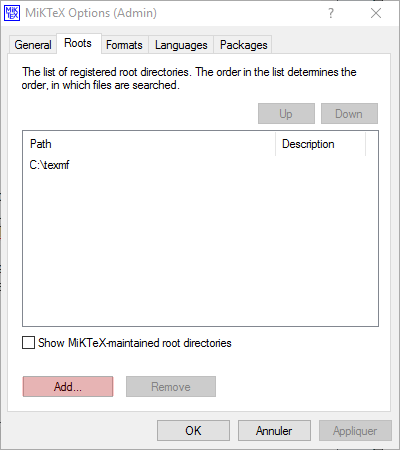
\includegraphics[scale=0.5]{MiKTeX-screenshot01.png}
\end{center}

\newpage

Dans l'onglet \og General \fg, vous pouvez maintenant cliquer sur le bouton \og Refresh FNDB \fg{} :
\begin{center}
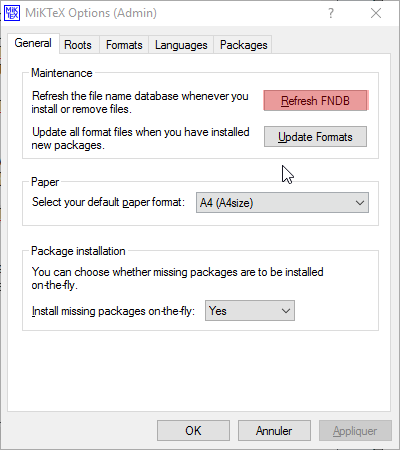
\includegraphics[scale=0.5]{MiKTeX-screenshot02.png}
\end{center}

Tant que vous êtes sur cet onglet, profitez-en pour vous assurer que le téléchargement des packages se fera automatiquement; pour cela, vérifiez que l'option \og Install missing packages on-the-fly \fg{} est à \og Yes \fg{} :
\begin{center}
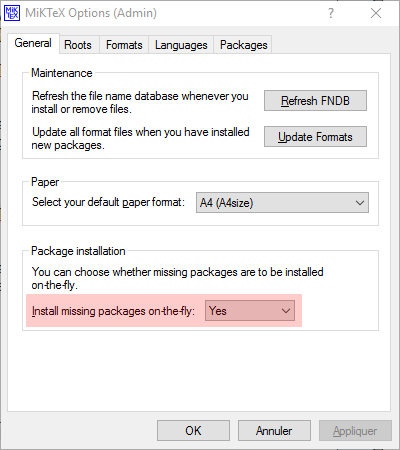
\includegraphics[scale=0.5]{MiKTeX-screenshot03.png}
\end{center}

\subsection{Rafraîchir la base de données sous Linux ou iOS}

Une fois l'arborescence créée ou/et les packages installés, lancez votre terminal (sous Windows, recherchez \og cmd \fg{} puis lancez-le). Exécutez alors la commande :

\begingroup
\color{white}
\begin{lstlisting}
texhash
\end{lstlisting}
\endgroup

Cela aura pour effet de rafraîchir la base de données de votre distribution \LaTeX.

\vspace*{1cm}

Vous êtes maintenant prêts pour explorer \texttt{pas-cours} !

\newpage

\section{Appel à l'extension}

\subsection{Les options}

\texttt{pas-cours} doit être appelé en préambule avec ou sans les options souhaitées :

\begingroup
\color{white}
\begin{lstlisting}
\documentclass[a4paper,french]{article}
...
\usepackage[<options>]{pas-cours}
\begin{document}
...
\end{document}
\end{lstlisting}
\endgroup

Il existe 6 options :

\begin{itemize}
\item \textbf{ant}, qui permet d'écrire les titres avec la police \texttt{anttlc} ;

\item \textbf{everytoc}, qui permet de mettre dans la table des matière (le sommaire) les titres de tous les environnements créés par \texttt{pas-cours} (théorèmes, définitions,...) ;

\item \textbf{noeffect}, qui supprime l'effet donné aux titres des environnements;

\item \textbf{notitlebreak}, voir page \pageref{notitlebreak} et \pageref{breakbox} pour plus de détails;

\item \textbf{noitemstyle}, qui aura pour effet de ne pas changer le styles des environnements \texttt{enumerate} et \texttt{itemize} (qui sont changés par défaut dès que \texttt{pas-cours} est appelé);

\item \textbf{calculs}, qui charge l'extension permettant de faire des calculs (voir page \pageref{calculs} pour plus de détails.
\end{itemize}

\subsection{Les extensions chargées}

\texttt{pas-cours} charge automatiquement les extensions suivantes :
\begin{itemize}
\item \textbf{amssymb}
\item \textbf{enumitem}
\item \textbf{fancyvrb}
\item \textbf{tikz} (avec les librairies \textit{calc}, \textit{arrows} et \textit{fadings})
\item \textbf{numprint}
\item \textbf{xkeyval}
\item \textbf{xstring}
\end{itemize}

\section{Titre des chapitres}


\begingroup
\color{white}
\begin{lstlisting}
\chap[<options>]{Titre du chapitre}{Sous-titre du chapitre}
\end{lstlisting}
\endgroup

Les options sont les suivantes :

\begin{itemize}
\item \textbf{autonum} : booléen (par défaut : false). Indique si le numéro de chapitre doit \^etre automatiquement calculé.
\item \textbf{num}, qui est le numéro du chapitre (obligatoire si \og autonum = false \fg.
\item \textbf{color}, qui est couleur que vous voulez; en cas d'absence, la couleur sera rouge).
\item \textbf{pos} = \textit{left} ou \textit{right}; en cas d'absence, la position du numéro du chapitre sera \og right \fg{} donc à droite).
\item \textbf{nonewpage}, qui est un booléen (par défaut : false). Indique si l'on ne souhaite pas mettre le titre sur une nouvelle page.
\end{itemize}

\begingroup
\color{white}
\begin{lstlisting}
\chap[num=1,color=blue,nonewpage]{Nombres entiers}{Stéphane PASQUET, \today}
\end{lstlisting}
\endgroup

donne : 

\chap[num=1,color=blue,nonewpage]{Nombres entiers}{Stéphane PASQUET, \today}

\section{La commande \textbackslash definmot}

Elle permet de mettre en relief un mot dans un cadre.

{\color{white}
\begin{lstlisting}
Un nombre est \definmot{premier} s'il n'est divisible que par 1 et lui-même.
\end{lstlisting}
}

donne :

\medskip

Un nombre est \definmot{premier} s'il n'est divisible que par 1 et lui-même.

\paragraph*{Remarque :} la couleur de l'argument de cette commande varie en fonction de l'environnement dans lequel elle est appelée : elle s'adapte à la couleur de l'environnement dans lequel elle se trouve.

\section{L'environnement \og pasbox \fg{} : l'environnement principal}
\label{pasbox}

\subsection{Syntaxe et options}

Cet environnement contient principalement les définitions, théorèmes, etc.

\medskip

{\color{white}
\begin{lstlisting}
\begin{pasbox}[<options>]
...
\end{pasbox}
\end{lstlisting}
}

Les options sont les suivantes :

\begin{enumerate}
\item Les booléens :
\begin{itemize}
\item \textbf{degrade} : si cette option est présente, le fond du cadre sera dégradé de la gauche vers la droite.

Par défaut, \texttt{degrade = true}.


\item \textbf{pluriel} : si cette option est présente, elle indique de mettre un \og s \fg{} à la fin du titre.

Par défaut, \texttt{pluriel=false}.


\item \textbf{num} : si cette option est présente, l'environnement sera numéroté. 

Par défaut, \texttt{num = false}.

\item \textbf{notitle} : si cette option est présente, le titre est supprimé.

Par défaut, \texttt{notitle = false}.

\item \textbf{notitlebreak} : si cette option est présente, si le cadre est coupé (avec l'option la commande \textbackslash breakbox), le titre dans le second cadre est supprimé.\label{notitlebreak}

À noter que si vous souhaitez utiliser cette option pour tous les environnements de votre document, cette option peut être présente dès l'appel de \texttt{pas-cours} (voir paragraphe 2 : \og Appel à l'extension \fg).

Par défaut, \texttt{notitlebreak=false}.

\item \textbf{endsymb} : si cette option est présente, un symbole sera affiché à la fin du texte de cet environnement. Quelques fois utilisé pour les démonstrations.

Par défaut, \texttt{endsymb=false}.

\item \textbf{toc} : si cette option est présente, le \texttt{name} de l'environnement actuel est inséré dans la table des matières.

Par défaut, \texttt{toc=false}.

\item \textbf{notoc} : si cette option est présente, le \texttt{name} de l'environnement actuel n'est pas inséré dans la table des matières.

Par défaut, \texttt{notoc=false}.

\item \textbf{effect} : si cette option est présente, un effet est mis sur le fond du titre de l'environnement.

Par défaut, \texttt{effect=true}.
\end{itemize}

\newpage

\item Les valeurs :
\begin{itemize}
\item \textbf{style=...} pour indiquer le contenu de l'environnement. Vous avez le choix entre les valeurs suivantes :
\begin{itemize}
\item defi (pour définition)
\item prop (pour propriété)
\item thm (pour théorème)
\item demo (pour démonstration)
\item nota (pour notation)
\item ex (pour exemple)
\item act (pour activité)
\item rem (pour remarque)
\item meth (pour méthode)
\end{itemize}

\item \textbf{name=...} pour indiquer le nom du cadre. Par exemple, \og name=Théorème de Pythagore \fg{} si vous énoncez ce théorème dans cet environnement.

\item \textbf{title=...}pour indiquer le titre de l'environnement. Par exemple, \og title=Propriété importante \fg{} si vous souhaitez ne pas voir comme titre : \og Propriété \fg{} avec le style \texttt{style=prop}.

\item \textbf{symb=...} pour indiquer un autre symbole que celui par défaut, c'est-à-dire : $\blacksquare$.
\end{itemize}
\end{enumerate}

\subsection{Exemples}

\subsubsection{Théorème non numéroté}

{\color{white}
\begin{lstlisting}
\begin{pasbox}[style=thm,name={Théorème de Pythagore},degrade]
Soit ABC un triangle rectangle en A. Alors, \[ BC^2=AB^2+AC^2\]
\end{pasbox}
\end{lstlisting}
}

\begin{pasbox}[style=thm,name={Théorème de Pythagore},degrade]
Soit ABC un triangle rectangle en A. Alors, \[ BC^2=AB^2+AC^2\]
\end{pasbox}

\subsubsection{Théorème numéroté}

{\color{white}
\begin{lstlisting}
\begin{pasbox}[style=thm,name={Théorème de Pythagore},degrade,num]
Soit ABC un triangle rectangle en A. Alors, \[ BC^2=AB^2+AC^2\]
\end{pasbox}
\end{lstlisting}
}

\begin{pasbox}[style=thm,name={Théorème de Pythagore},degrade,num]
Soit ABC un triangle rectangle en A. Alors, \[ BC^2=AB^2+AC^2\]
\end{pasbox}

\subsubsection{Définition sans titre mais avec un nom}

{\color{white}
\begin{lstlisting}
\begin{pasbox}[style=defi,name=Centre de gravité,degrade,notitle]
Dans un triangle, le point d'intersection des médianes est appelé le \definmot{centre de gravité}.
\end{pasbox}
\end{lstlisting}
}

\begin{pasbox}[style=defi,name=Centre de gravité,degrade,notitle]
Dans un triangle, le point d'intersection des médianes est appelé le \definmot{centre de gravité}.
\end{pasbox}


\subsubsection{Définitions (au pluriel et avec un titre)}

{\color{white}
\begin{lstlisting}
\begin{pasbox}[style=defi,pluriel]
Dans un triangle, une droite passant par un sommet et par le milieu du côté opposé est appelée une \definmot{médiane}.

Une droite passant par un sommet et perpendiculaire au coté opposé est appelée une \definmot{hauteur}.
\end{pasbox}
\end{lstlisting}
}

\begin{pasbox}[style=defi,pluriel]
Dans un triangle, une droite passant par un sommet et par le milieu du côté opposé est appelée une \definmot{médiane}.

Une droite passant par un sommet et perpendiculaire au coté opposé est appelée une \definmot{hauteur}.
\end{pasbox}

Notez la présence ici de la commande \texttt{\textbackslash definmot}, définie dans ce package, pour mettre en valeur un mot, et sa couleur... qui est adaptée à l'environnement.

\subsubsection{Propriété}

{\color{white}
\begin{lstlisting}
\begin{pasbox}[style=prop]
Dans un triangle, les trois médianes sont concourantes.
\end{pasbox}
\end{lstlisting}
}

\begin{pasbox}[style=prop]
Dans un triangle, les trois médianes sont concourantes.
\end{pasbox}

\subsubsection{Exemple}

{\color{white}
\begin{lstlisting}
\begin{pasbox}[style=ex,pluriel]
\begin{enumerate}
\item $x+2=9$ donc $x=9-2$, soit $x=7$.
\item $x-3=4$ donc $x=4+3$, soit $x=7$.
\end{enumerate} 
\end{pasbox}
\end{lstlisting}
}

\begin{pasbox}[style=ex,pluriel]
\begin{enumerate}
\item $x+2=9$ donc $x=9-2$, soit $x=7$.
\item $x-3=4$ donc $x=4+3$, soit $x=7$.
\end{enumerate} 
\end{pasbox}

Notez ici que la couleur des numéros devant chaque ligne s'adapte à l'environnement.

\newpage

\subsubsection{Notations}

{\color{white}
\begin{lstlisting}
\begin{pasbox}[style=nota,pluriel]
\begin{enumerate}
\item $x \times x$ est noté $x^2$.
\item $x+x$ est noté $2x$.
\item $x+x+x$ est noté $3x$.
\end{enumerate}
\end{pasbox}
\end{lstlisting}
}

\begin{pasbox}[style=nota,pluriel]
\begin{enumerate}
\item $x \times x$ est noté $x^2$.
\item $x+x$ est noté $2x$.
\item $x+x+x$ est noté $3x$.
\end{enumerate}
\end{pasbox}

\subsubsection{Remarque}

{\color{white}
\begin{lstlisting}
\begin{pasbox}[style=rem,name=Note historique]
Le symbole \og $\times$ \fg{} a été introduit par William OUGHTRED (1574 - 1660).
\end{pasbox}
\end{lstlisting}
}

\begin{pasbox}[style=rem,name=Note historique]
Le symbole \og $\times$ \fg{} a été introduit par William OUGHTRED (1574 - 1660).
\end{pasbox}

\subsubsection{Activité}

{\color{white}
\begin{lstlisting}
\begin{pasbox}[style=act,name=Propriétés sur les droites]
\begin{enumerate}
\item Tracez deux droites perpendiculaires $(d)$ et $(d')$.
\item Tracez une droite $(d'')$ perpendiculaire à $(d)$.
\item Comment semble être $(d'')$ par rapport à $(d')$ ?
\end{enumerate}
\end{pasbox} 
\end{lstlisting}
}

\begin{pasbox}[style=act,name=Propriétés sur les droites]
\begin{enumerate}
\item Tracez deux droites perpendiculaires $(d)$ et $(d')$.
\item Tracez une droite $(d'')$ perpendiculaire à $(d)$.
\item Comment semble être $(d'')$ par rapport à $(d')$ ?
\end{enumerate}
\end{pasbox} 

\newpage

\subsubsection{Méthode}

{\color{white}
\begin{lstlisting}
\begin{pasbox}[style=meth,name=Trouver la forme irréductible d'une fraction,endsymb,symb=$\bigstar$]
Pour simplifier au maximum la fraction $\dfrac{\numprint{29700}}{\numprint{35100}}$, on décompose en produit de facteurs premiers le numérateur et le dénominateur :
\[
\dfrac{\numprint{29700}}{\numprint{35100}}=\dfrac{2^2\times3^3\times5^5\times11}{2^2\times3^3\times5^5\times13}=\dfrac{11}{13}.
\]
\end{pasbox}
\end{lstlisting}
}


\begin{pasbox}[style=meth,name=Trouver la forme irréductible d'une fraction,endsymb,symb=$\bigstar$]
Pour simplifier au maximum la fraction $\dfrac{\numprint{29700}}{\numprint{35100}}$, on décompose en produit de facteurs premiers le numérateur et le dénominateur :
\[
\dfrac{\numprint{29700}}{\numprint{35100}}=\dfrac{2^2\times3^3\times5^5\times11}{2^2\times3^3\times5^5\times13}=\dfrac{11}{13}.
\]
\end{pasbox}

\subsubsection{Démonstration}

{\color{white}
\begin{lstlisting}
\begin{pasbox}[name=Théorème de Pythagore,endsymb,title=Démonstration,style=demo]
Ici, on rédige la preuve du théorème de Pythagore.\\
C'est un peu long...
\end{pasbox}
\end{lstlisting}
}

\begin{pasbox}[name=Théorème de Pythagore,endsymb,title=Démonstration,style=demo]
Ici, on rédige la preuve du théorème de Pythagore.\\
C'est un peu long...
\end{pasbox}

\subsection{Nom avec virgule}

Si vous souhaitez mettre en argument un groupe de mots séparés par des virgules, il faut mettre ce groupe de mots entre accolades.

{\color{white}
\begin{lstlisting}
\begin{pasbox}[style=defi,pluriel,name={dixièmes, centièmes et millièmes}]
On insère ici les définitions.
\end{pasbox}
\end{lstlisting}
}

\begin{pasbox}[style=defi,pluriel,name={dixièmes, centièmes et millièmes}]
On insère ici les définitions.
\end{pasbox}

\newpage

\subsection{Définition d'un autre style}

Je n'ai pas pu mettre tous les styles de cadres possibles, mais uniquement les plus répandus.

Cependant, on peut définir soit-même son cadre \og Corollaire \fg{} par exemple :

{\color{white}
\begin{lstlisting}
\definecolor{macouleur}{cmyk}{0,0.27,0.03,0}
\newenvironment{corollaire}[1][]
{%
\begin{pasbox}[degrade,color=macouleur,title=Corollaire,name={#1}]
}
{%
\end{pasbox}
}
\begin{corollaire}[Relatif à la propriété 2]
Mon corollaire ici.
\end{corollaire}
\end{lstlisting}
}

\definecolor{macouleur}{cmyk}{0,0.27,0.03,0}
\newenvironment{corollaire}[1][]
{%
\begin{pasbox}[degrade,color=macouleur,title=Corollaire,name={#1}]
}
{%
\end{pasbox}
}
\begin{corollaire}[Relatif à la propriété 2]
Mon corollaire ici.
\end{corollaire}

\subsection{Cassage d'un cadre : la commande \textbackslash breakbox}
\label{breakbox}

L'environnement \texttt{pasbox} n'est pas en mesure de couper automatiquement les cadres si ceux-ci sont en bas de page; il faut le faire manuellement de la manière suivante :

{\color{white}
\begin{lstlisting}
\begin{pasbox}[style=ex,pluriel,degrade,name={Théorème de Pythagore},effect=false]
ABC est un triangle rectangle en A tel que $\text{AB}=5$ et $\text{AC}=7$.

On a alors :
\begin{align*}
BC^2 & = AB^2+AC^2\\
BC^2& = 74
\end{align*}
\breakbox
De même, dans le triangle BCD rectangle en D, avec $\text{BD}=6$, on a :
\begin{align*}
CD^2 & = BD^2+BC^2\\
CD^2 & = 36+74\\
CD^2 & = 110
\end{align*}
\end{pasbox}
\end{lstlisting}
}

\begin{pasbox}[style=ex,pluriel,degrade,name={Théorème de Pythagore},effect=false]
ABC est un triangle rectangle en A tel que $\text{AB}=5$ et $\text{AC}=7$.

On a alors :
\begin{align*}
BC^2 & = AB^2+AC^2\\
BC^2& = 74
\end{align*}
\breakbox
De même, dans le triangle BCD rectangle en D, avec $\text{BD}=6$, on a :
\begin{align*}
CD^2 & = BD^2+BC^2\\
CD^2 & = 36+74\\
CD^2 & = 110
\end{align*}
\end{pasbox}


\paragraph*{N.B.} Dans l'éventualité où vous souhaiteriez enlever le titre de la seconde boîte, utilisez l'option \texttt{notitlebreak} :

\medskip

{\color{white}
\begin{lstlisting}
\begin{pasbox}[style=ex,notitlebreak]
Premier cadre
\breakbox
Second cadre
\end{pasbox}
\end{lstlisting}
}

\begin{pasbox}[style=ex,notitlebreak]
Premier cadre
\breakbox
Second cadre
\end{pasbox}

\paragraph*{Remarque :} si vous mettez l'option \texttt{notitle}, il n'y aura pas de titre au 1\ier{} et 2\ieme{} cadre.

\section{Insérer une entrée dans la table des matières}

Par défaut, rien n'est inséré dans la table des matières.

Si l'on veut qu'il n'en soit pas ainsi, on utilisera l'option \texttt{toc} comme dans l'exemple suivant :

{\color{white}
\begin{lstlisting}
\begin{pasbox}[style=thm,name=Pythagore,toc]
Si un triangle ABC est rectangle en A, alors :
\[ BC^2=AB^2+AC^2.\]
\end{pasbox}
\end{lstlisting}
}

\medskip

Si l'on veut que tous les environnements figurent dans la table des matières, on fera appel au package avec l'option \texttt{everytoc} :

\medskip


{\color{white}
\begin{lstlisting}
\usepackage[everytoc]{pas-cours}
\end{lstlisting}
}

Dans ce cas, tous les environnements où \texttt{name} sera informé, \texttt{name} sera inséré dans la table des matières.


\bigskip

Si on ne souhaite pas qu'un \texttt{name} figure dans cette table, on utilisera l'option \texttt{notoc}.


{\color{white}
\begin{lstlisting}
\begin{pasbox}[style=prop,notoc]
La, je suis sûr que cette boîte ne figurera pas dans la TOC.
\end{pasbox}
\end{lstlisting}
}


\newpage

\section{Environnements \og \`A retenir \fg, \og Attention \fg{} et\\ \og Prérequis \fg{}  }

\subsection{\`A retenir}

{\color{white}
\begin{lstlisting}
\begin{aretenir}[0.5]
\lipsum[1]
\end{aretenir}
\end{lstlisting}
}

\begin{aretenir}[0.5]
\lipsum[1]
\end{aretenir}


Le nombre entre crochets est un coefficient pour agrandir ou réduire la taille de l'image.

L'image affichée se nomme \og coeur.png \fg{} ; elle se trouve dans le répertoire d'installation du package \texttt{pas-cours.sty}.

\subsection{Attention}

{\color{white}
\begin{lstlisting}
\begin{attention}[0.5]
\lipsum[1]
\end{attention}
\end{lstlisting}
}

\begin{attention}[0.5]
\lipsum[1]
\end{attention}

Le nombre entre crochets est un coefficient pour agrandir ou réduire la taille de l'image.

L'image affichée se nomme \og attention.png \fg{} ; elle se trouve dans le répertoire d'installation du package \texttt{pas-cours.sty}.

\medskip

Après avoir remarqué que cet environnement ne fonctionnait pas selon le mode de compilation, j'ai créé un autre environnement plus souple :

{\color{white}
\begin{lstlisting}
\begin{warning}[scale=0.05,img=warning-perso.png,margins=1em,bg,bgcolor=blue!10,draw=blue!50!black]
Ceci est le nouvel environnement en date du 29 avril 2015.
\end{warning}
\end{lstlisting}
}

\begin{warning}[scale=0.05,img=warning-perso.png,margins=1em,bg,bgcolor=blue!10,draw=blue!50!black]
Ceci est le nouvel environnement en date du 29 avril 2015.
\end{warning}

Cet environnement comporte les options suivantes :

\begin{itemize}
\item \texttt{scale} : l'échelle de l'image affichée ;
\item \texttt{img} : nom de l'image souhaitée (doit être dans le répertoire courant) ;
\item \texttt{margins} : marges internes ;
\item \texttt{draw} : couleur du cadre  (par défaut : red!50!black) ;
\item \texttt{bg} : booléen (par défaut : false) ;
\item \texttt{bgcolor} : couleur de fond (si \texttt{bg=true}).
\end{itemize}

\subsection{Prérequis}

{\color{white}
\begin{lstlisting}
\begin{prerequis}
\item Prérequis 1
\item Prérequis 2
\end{prerequis}
\end{lstlisting}
}

\begin{prerequis}
\item Prérequis 1
\item Prérequis 2
\end{prerequis}


\section{Commande \og bonus \fg{} }

Cette commande s'utilise généralement en fin de chapitre, lorsque l'enseignant(e) souhaite insérer des fiches.

\medskip

{\color{white}
\begin{lstlisting}
\bonus{Titre} % Insère le titre dans le sommaire
\bonus*{Titre} % N'insère pas le titre dans le sommaire
\end{lstlisting}
}

Elle exécute un saut de page (en appelant la commande \texttt{\textbackslash newpage}), puis insère un titre sous la forme \og Complément <num> : Titre \fg{} (les numéros sont automatiquement calculés). Voir page suivante.

\bonus*{Ici, ma fiche}

\newpage

\section{Styles des listes}

Par défaut, le style des listes a changé :

\medskip\itemclass{black}


{\color{white}
\begin{lstlisting}
\begin{enumerate}
\item Item 1
\item Item 2
\end{enumerate}
\end{lstlisting}
}

donne :

\begin{enumerate}
\item Item 1
\item Item 2
\end{enumerate}


{\color{white}
\begin{lstlisting}
\begin{itemize}
\item Item 1
\item  Item 2
\begin{itemize}
\item Sous-Item 1
\end{itemize}
\end{itemize}
\end{lstlisting}
}

donne :

\begin{itemize}
\item Item 1
\item  Item 2
\begin{itemize}
\item Sous-Item 1
\end{itemize}
\end{itemize}

\medskip

La couleur varie en fonction de l'environnement dans lequel est la liste.

Pour changer la couleur, on peut utiliser la commande \texttt{\textbackslash itemclass\{<couleur>\}} :

\medskip

{\color{white}
\begin{lstlisting}
\itemclass{red}
\begin{enumerate}
\item Item 1
\end{enumerate}
\itemclass{blue}
\begin{enumerate}[start=2]
\item Item 2
\end{enumerate}
\end{lstlisting}
}

\itemclass{red}
\begin{enumerate}
\item Item 1
\end{enumerate}
\itemclass{blue}
\begin{enumerate}[start=2]
\item Item 2
\end{enumerate}

\bigskip

Dans l'éventualité où ces styles ne vous plaisent pas, vous pouvez toujours utiliser les outils du package \texttt{enumitem} pour les changer (dans ce cas, reportez-vous à sa documentation).

\medskip

Mais si vous ne souhaitez pas que le style des listes change par défaut, faites appel à \texttt{pas-cours} avec l'option \texttt{noitemstyle}:

{\color{white}
\begin{lstlisting}
\usepackage[noitemstyle]{pas-cours}
\end{lstlisting}
}

\newpage

\section{Figures usuelles dans l'espace}


\subsection{Le cube et le parallélépipède rectangle}

\subsubsection{Syntaxe}

{\color{white}
\begin{lstlisting}
\begin{tikzpicture}
\cube[<options>]
\end{tikzpicture}
\end{lstlisting}
}

Les options sont les suivantes :

\begin{itemize}
\item \textbf{bordercolor=} couleur du bord.

Par défaut, elle sera noire.


\item \textbf{incolor=} couleur des faces.

Par défaut, elle sera blanche.


\item \textbf{angle=} angle (en degré) de la perspective.

Par défaut, il sera de 45$^\circ$.


\item \textbf{scale=}  coefficient d'agrandissement ou de réduction.

Par défaut, l'arête du cube est égale à 1~cm.


\item \textbf{coefopaq=} coefficient d'opacité, entre 0 et 1.

Par défaut, il vaut 0,5.


\item \textbf{prof=}  la profondeur du parallélépipède rectangle.

Par défaut, elle vaut 1.


\item \textbf{name}  :   option booléenne ; si elle ne paraît pas, la figure sera sans nom.

\item \textbf{legende} : option booléenne ; si elle ne paraît pas, la légende de la figure ne sera pas écrite.
\end{itemize}

\subsubsection{Exemple 1 : avec légende}

{\color{white}
\begin{lstlisting}
\begin{tikzpicture}
\cube[bordercolor=orange,incolor=green!50!black,angle=30, coefopaq=0.2,scale=3,
name,legende]
\end{tikzpicture}
\end{lstlisting}
}

\begin{center}
\begin{tikzpicture}
\cube[bordercolor=orange,incolor=green!50!black,angle=30, coefopaq=0.2,scale=3,
name,legende]
\end{tikzpicture}
\end{center}

\newpage

\subsubsection{Exemple 2 : sans légende}

{\color{white}
\begin{lstlisting}
\begin{tikzpicture}
\cube[bordercolor=blue,incolor=blue,angle=45,coefopaq=0.3,scale=2]
\end{tikzpicture}
\end{lstlisting}
}

\begin{center}
\begin{tikzpicture}
\cube[bordercolor=blue,incolor=blue,angle=45,coefopaq=0.3,scale=2]
\end{tikzpicture}
\end{center}

\subsubsection{Exemple 3 : parallélépipède rectangle}

{\color{white}
\begin{lstlisting}
\begin{tikzpicture}
\cube[bordercolor=purple,incolor=purple,angle=30,scale=2,prof=3,coefopaq=0.2]
\end{tikzpicture}
\end{lstlisting}
}

\begin{center}
\begin{tikzpicture}
\cube[bordercolor=purple,incolor=purple,angle=30,scale=2,prof=3,coefopaq=0.2]
\end{tikzpicture}
\end{center}

\subsection{Le cône de révolution}


\subsubsection{Syntaxe}

{\color{white}
\begin{lstlisting}
\begin{tikzpicture}
\cone[<options>]
\end{tikzpicture}
\end{lstlisting}
}

Les options sont les suivantes :

\begin{itemize}
\item \textbf{bordercolor=} couleur du bord.

Par défaut, elle sera noire.

\item \textbf{incolor=} couleur des faces.

Par défaut, elle sera blanche.

\item \textbf{incl=} coefficient d'inclinaison du disque de base.

Par défaut, égal à 0,33.

\item \textbf{hauteur=} hauteur du cône.

Par défaut, elle vaut 3 cm.

\item \textbf{coefopaq=} coefficient d'opacité, compris entre 0 et 1.

Par défaut, il vaut 0,5.

\item \textbf{rayon=} rayon du disque de base.

Par défaut, il faut 1 cm.

\item \textbf{centre=} nom du centre du disque de base.

Par défaut, il est nommé O.

\item \textbf{poscentre=} position du nom du centre du disque de base (en langage TikZ : \textit{above}, \textit{below}, \textit{
below right}, ...).

Par défaut : below.

\item \textbf{sommet=} nom du sommet du cône.

Par défaut, il est nommé : S.

\item \textbf{posommet=}  position du nom du sommet.

Par défaut : above.


\item \textbf{scalecentre=} coefficient d'agrandissement du point représentant le centre du disque de base.

\item \textbf{name} :  option booléenne ; si elle ne paraît pas, la figure sera sans nom.

\item \textbf{axe} : option booléenne ; si elle ne paraît pas, l'axe de révolution ne sera pas dessiné.

\item \textbf{axecolor=} couleur de l'axe de révolution.

Par défaut, il est rouge.

\item \textbf{legende} : option booléenne ; si elle ne paraît pas, la légende de la figure ne sera pas mise.
\end{itemize}

\subsubsection{Exemple 1 : sans option}

{\color{white}
\begin{lstlisting}
\begin{tikzpicture}
\cone
\end{tikzpicture}
\end{lstlisting}
}

\begin{center}
\begin{tikzpicture}
\cone
\end{tikzpicture}
\end{center}

\subsubsection{Exemple 2 : avec deux points}

{\color{white}
\begin{lstlisting}
\begin{tikzpicture}
\cone[incolor=purple,bordercolor=purple,coefopaq=0.3,incl=0.1,rayon=3,hauteur=3,name,sommet=A,centre=B,poscentre=right,scalecentre=3]
\end{tikzpicture}
\end{lstlisting}
}

\begin{center}
\begin{tikzpicture}
\cone[incolor=purple,bordercolor=purple,coefopaq=0.3,incl=0.1,rayon=3,hauteur=3,
name,sommet=A,centre=B,poscentre=right,scalecentre=3]
\end{tikzpicture}
\end{center}

\newpage

\subsubsection{Exemple 3 : avec légende}

{\color{white}
\begin{lstlisting}
\begin{tikzpicture}
\cone[incolor=green,coefopaq=0.3,rayon=3,hauteur=3,name,sommet=A,centre=B,axe,
legende,posommet={above right},poscentre=right,incl=0.1,scalecentre=3]
\end{tikzpicture}
\end{lstlisting}
}

\begin{center}
\begin{tikzpicture}
\cone[incolor=green,coefopaq=0.3,rayon=3,hauteur=3,name,sommet=A,centre=B,axe,
legende,posommet={above right},poscentre=right,incl=0.1,scalecentre=3]
\end{tikzpicture}
\end{center}


\subsection{Le cylindre de révolution}

\subsubsection{Syntaxe}

{\color{white}
\begin{lstlisting}
\begin{tikzpicture}
\cylindre[<options>]
\end{tikzpicture}
\end{lstlisting}
}

Les options sont les suivantes :

\begin{itemize}
\item \textbf{bordercolor=} couleur du bord.

Par défaut, elle sera noire.


\item \textbf{incolor=} couleur des faces.

Par défaut, elle sera blanche.


\item \textbf{incl=} coefficient d'inclinaison du disque de base.

Par défaut, égal à 0,33.


\item \textbf{hauteur=}  hauteur du cône.

Par défaut, elle vaut 3 cm.


\item \textbf{coefopaq=} coefficient d'opacité compris entre 0 et 1.

Par défaut, il vaut 0,5.


\item \textbf{rayon=} rayon (en cm) du disque de base.

Par défaut, il faut 1 cc.


\item \textbf{centrehaut=} nom du centre du disque du haut.

Par défaut, il est nommé : H.


\item \textbf{poscentrehaut=} position du nom du centre du disque du haut (above, right, left, below, below left,...).

Par défaut : below.


\item \textbf{centrebas=}  nom du centre du disque du bas.

Par défaut, il est nommé : B.


\item \textbf{poscentrebas=} position du nom du centre du disque de base.

Par défaut : below.


\item \textbf{scalecentre=}  coefficient d'agrandissement du point représentant le centre du disque de base.

\item \textbf{name}  :  option booléenne ; si elle ne paraît pas, la figure sera sans nom.

\item \textbf{axe} : option booléenne ; si elle ne paraît pas, l'axe de révolution ne sera pas dessiné.

\item \textbf{axecolor=} couleur de l'axe de révolution.

Par défaut, il est rouge.

\item \textbf{legende}  :   option booléenne ; si elle ne paraît pas, la légende de la figure ne sera pas mise.

\item \textbf{rectgener}  :  option booléenne ; si elle ne paraît pas, le rectangle générateur ne sera pas tracé.
\end{itemize}

\subsubsection{Exemple 1 : sans option}

{\color{white}
\begin{lstlisting}
\begin{tikzpicture}
\cylindre
\end{tikzpicture}
\end{lstlisting}
}

\begin{center}
\begin{tikzpicture}
\cylindre
\end{tikzpicture}
\end{center}

\subsubsection{Exemple 2 : avec deux points}

{\color{white}
\begin{lstlisting}
\begin{tikzpicture}
\cylindre[incolor=purple,bordercolor=purple,coefopaq=0.3,incl=0.1,rayon=3,
hauteur=3,name,centrehaut=A,poscentrehaut=left,poscentrebas=left,
scalecentre=3]
\end{tikzpicture}
\end{lstlisting}
}

\begin{center}
\begin{tikzpicture}
\cylindre[incolor=purple,bordercolor=purple,coefopaq=0.3,incl=0.1,rayon=3,
hauteur=3,name,centrehaut=A,poscentrehaut=left,poscentrebas=left,
scalecentre=3]
\end{tikzpicture}
\end{center}

\newpage

\subsubsection{Exemple 3 : avec légende}

{\color{white}
\begin{lstlisting}
\begin{tikzpicture}
\cylindre[incolor=blue,bordercolor=red,coefopaq=0.2,name,legende,rectgener,axe,
poscentrehaut=left,poscentrebas=left,scalecentre=3]
\end{tikzpicture}
\end{lstlisting}
}

\begin{center}
\begin{tikzpicture}
\cylindre[incolor=blue,bordercolor=red,coefopaq=0.2,name,legende,rectgener,axe,
poscentrehaut=left,poscentrebas=left,scalecentre=3]
\end{tikzpicture}
\end{center}

\subsection{Sphère et boule}

\subsubsection{Syntaxe}

{\color{white}
\begin{lstlisting}
\begin{tikzpicture}
\boule[<options>]
\end{tikzpicture}
\end{lstlisting}
}

Les options sont les suivantes :

\begin{itemize}
\item \textbf{border} : option booléenne; si mentionnée, le bord de la boule (la sphère) est dessiné.

\item \textbf{bordercolor=} couleur du bord.

Par défaut, elle sera noire.


\item \textbf{incolor=} couleur de la boule.

Par défaut, elle sera blanche.


\item \textbf{coefopaq=} coefficient d'opacité compris entre 0 et 1.

Par défaut, il vaut 0,5.

\item \textbf{centre=} nom du centre de la boule.

Par défaut, il est nommé : O.

\item \textbf{poscentre=} position du centre de la boule.

Par défaut : below.

\item \textbf{scale=}  coefficient d'agrandissement de la boule.

\item \textbf{name} : option booléenne ; si elle ne paraît pas, le centre ne sera pas dessiné.

\item \textbf{legende}  : option booléenne ; si elle ne paraît pas, la légende ne sera pas mise.

\item \textbf{greenwich}  :  option booléenne ; si elle paraît, le méridien de Greenwich est tracé.

\item \textbf{greenwichcolor=} couleur du méridien de Greenwich.

\item \textbf{greenwichlegende}  : option booléenne ; si elle paraît, la légende du méridien de Greenwich apparaît.

\item \textbf{grandcercle} : option booléenne ; si elle paraît, l'équateur sera dessiné.

\item \textbf{equateurlegende}  : option booléenne ; si elle paraît, la légende sera mise pour l'équateur.

\item \textbf{exemplecoord}  :  option booléenne ; si elle paraît, un exemple de coordonnées sphériques est tracé.

\item \textbf{exemplecoordcolor}  :  couleur dominante de l'exemple (par défaut, vert foncé).

\item \textbf{exemplecoordname} : nom du point dans l'exemple. 

Par défaut, \og A \fg.
\end{itemize}

\subsubsection{Exemple 1 : sans option}

{\color{white}
\begin{lstlisting}
\begin{tikzpicture}
\boule
\end{tikzpicture}
\end{lstlisting}
}

\begin{center}
\begin{tikzpicture}
\boule
\end{tikzpicture}
\end{center}

\subsubsection{Exemple 2 : avec grands cercles}

{\color{white}
\begin{lstlisting}
\begin{tikzpicture}
\boule[grandcercle,name,incolor=blue, bordercolor=blue,legende]
\end{tikzpicture}
\end{lstlisting}
}

\begin{center}
\begin{tikzpicture}
\boule[grandcercle,name,incolor=blue, bordercolor=blue,legende]
\end{tikzpicture}
\end{center}

\subsubsection{Exemple 3 : sphère}

{\color{white}
\begin{lstlisting}
\begin{tikzpicture}
\boule[coefopaq=0,border,grandcercle,name,poscentre={below right}]
\end{tikzpicture}
\end{lstlisting}
}

\begin{center}
\begin{tikzpicture}
\boule[coefopaq=0,border,grandcercle,name,poscentre={below right}]
\end{tikzpicture}
\end{center}

\newpage

\subsubsection{Exemple 4 : coordonnées sphériques}

{\color{white}
\begin{lstlisting}
\begin{tikzpicture}
\boule[grandcercle,greenwich,greenwichcolor=red,greenwichlegende,border,equateurlegende,name,poscentre=above left,exemplecoord,coefopaq=0]
\end{tikzpicture}

La longitude de A est:$80^\circ$.\\La latitude de A est:$40^\circ$.
\end{lstlisting}
}

\begin{center}
\begin{tikzpicture}
\boule[grandcercle,greenwich,greenwichcolor=red,greenwichlegende,border,equateurlegende,name,poscentre=above left,exemplecoord,coefopaq=0]
\end{tikzpicture}
\end{center}

La longitude de A est:$80^\circ$.\\La latitude de A est:$40^\circ$.



\subsection{Pyramide à base régulière}

\subsubsection{Syntaxe}

{\color{white}
\begin{lstlisting}
\begin{tikzpicture}
\pyramreg[<options>]
\end{tikzpicture}
\end{lstlisting}
}

Les options sont les suivantes :

\begin{itemize}
\item \textbf{n=} nombre de côtés de la base.

Par défaut : 3.

\item \textbf{bordercolor=} couleur du bord.

Par défaut, elle sera noire.

\item \textbf{incolor=} couleur de la boule.

Par défaut, elle sera blanche.

\item \textbf{coefopaq=} coefficient d'opacité compris entre 0 et 1.

Par défaut, il vaut 0,5.

\item \textbf{centre=} nom du centre de la base.

Par défaut, il est nommé : O.

\item \textbf{poscentre=} position du centre de la boule. Possibilités : below, left, right, above, above right, above left, below right et below left.

Par défaut : below.
	
\item \textbf{sommet=} nom du sommet.

Par défaut, il est nommé : S.

\item \textbf{posommet=} position du nom du sommet.

Par défaut : above.


\item \textbf{scalecentre=} coefficient d'agrandissement du point représentant le centre de la base.

\item \textbf{axe} : option booléenne ; si elle ne figure pas, l'axe de rotation ne sera pas tracé.

\item \textbf{axecolor=} couleur de l'axe de rotation.

Par défaut : rouge.

\item \textbf{name} : option booléenne ; si elle ne paraît pas, le centre de la base et le nom des points ne sera pas mis.

\item \textbf{hauteur=} hauteur (en cm) du sommet.

Par défaut : 5 cm.

\item \textbf{rayon=} rayon (en cm) du cercle circonscrit à la base.

Par défaut : 2 cm.

\item \textbf{incl=} coefficient d'inclinaison de la base.

\item \textbf{legende} : option booléenne ; si elle ne paraît pas, la légende ne sera pas mise.

\item \textbf{rotat=} angle (en degré) de rotation de la vue (par défaut, il est nul).
\end{itemize}


\subsubsection{Exemple 1 : sans option}

{\color{white}
\begin{lstlisting}
\begin{tikzpicture}
\pyramreg
\end{tikzpicture}
\end{lstlisting}
}

\begin{center}
\begin{tikzpicture}
\pyramreg
\end{tikzpicture}
\end{center}

\subsubsection{Exemple 2}

{\color{white}
\begin{lstlisting}
\begin{tikzpicture}[scale=0.8,every node/.style={scale=0.8}]
\pyramreg[n=6,axe,name,posommet={above right}, poscentre=right, incolor=green!50!black, bordercolor=green!50!black, hauteur=3, rayon=3, scalecentre=5, poscentre=left,legende]
\end{tikzpicture}
\end{lstlisting}
}

\begin{center}
\begin{tikzpicture}[scale=0.8,every node/.style={scale=0.8}]
\pyramreg[n=6,axe,name,posommet={above right}, poscentre=right, incolor=green!50!black, bordercolor=green!50!black, hauteur=3, rayon=3, scalecentre=5, poscentre=left,legende]
\end{tikzpicture}
\end{center}

\newpage

\subsubsection{Exemple 3}

{\color{white}
\begin{lstlisting}
\begin{tikzpicture}
\pyramreg[n=5,incolor=blue,bordercolor=red,hauteur=4,incl=0.5]
\end{tikzpicture}
\end{lstlisting}
}

\begin{center}
\begin{tikzpicture}
\pyramreg[n=5,incolor=blue,bordercolor=red,hauteur=4,incl=0.5]
\end{tikzpicture}
\end{center}

\subsubsection{Exemple 4}

{\color{white}
\begin{lstlisting}
\begin{tikzpicture}
\pyramreg[n=13,coefopaq=0,name]
\end{tikzpicture}
\end{lstlisting}
}

\begin{center}
\begin{tikzpicture}
\pyramreg[n=13,coefopaq=0,name]
\end{tikzpicture}
\end{center}


\subsection{Prisme à base régulière}

\subsubsection{Syntaxe}

{\color{white}
\begin{lstlisting}
\begin{tikzpicture}
\prismereg[<options>]
\end{tikzpicture}
\end{lstlisting}
}

Les options sont les suivantes :

\begin{itemize}
\item \textbf{n=} nombre de côtés de la base (par défaut : 3).
\item \textbf{bordercolor=} couleur du bord (par défaut, elle sera noire).
\item \textbf{incolor=} couleur de la boule (par défaut, elle sera blanche).
\item \textbf{coefopaq=} coefficient d'opacité compris entre 0 et 1 (par défaut, il vaut 0,5).
\item \textbf{axe} :  option booléenne ;  si elle ne figure pas, l'axe de rotation ne sera pas tracé.
\item \textbf{axecolor=} couleur de l'axe de rotation (par défaut : rouge).
\item \textbf{hauteur=} hauteur (en cm) du sommet (par défaut : 5 cm).
\item \textbf{rayon=} rayon (en cm) du cercle circonscrit à la base (par défaut : 2 cm).
\item \textbf{incl=} coefficient d'inclinaison de la base.
\item \textbf{legende} : option booléenne ; si elle ne paraît pas, la légende ne sera pas mise.
\item \textbf{rotat=} angle de rotation de la vue (par défaut, il est nul sauf pour n=3 où il est égal à 10$^{\circ}$).
\item \textbf{name} :  option booléenne ; si elle ne paraît pas, le nom des points ne figurera pas.
\end{itemize}


\subsubsection{Exemple 1}

{\color{white}
\begin{lstlisting}
\begin{tikzpicture}
\prismereg[hauteur=2]
\end{tikzpicture}
\end{lstlisting}
}

\begin{center}
\begin{tikzpicture}
\prismereg[hauteur=2]
\end{tikzpicture}
\end{center}

\subsubsection{Exemple 2}


{\color{white}
\begin{lstlisting}
\begin{tikzpicture}
\prismereg[n=5,rotat=20,incolor=blue,bordercolor=red,rayon=3,hauteur=2,name]
\end{tikzpicture}
\end{lstlisting}
}

\begin{center}
\begin{tikzpicture}
\prismereg[n=5,rotat=20,incolor=blue,bordercolor=red,rayon=3,hauteur=2,name]
\end{tikzpicture}
\end{center}

\newpage

\subsubsection{Exemple 3}

{\color{white}
\begin{lstlisting}
\begin{tikzpicture}[scale=0.8,every node/.style={scale=0.8}]
\prismereg[n=6,coefopaq=0,incl=0.2,rotat=20,legende,incolor=black,axe]
\end{tikzpicture}
\end{lstlisting}
}

\begin{center}
\begin{tikzpicture}[scale=0.8,every node/.style={scale=0.8}]
\prismereg[n=6,coefopaq=0,incl=0.2,rotat=20,legende,incolor=black,axe]
\end{tikzpicture}
\end{center}

\section{Patrons de figures}

\subsection{Pavé droit}

\subsubsection{Syntaxe}

{\color{white}
\begin{lstlisting}
\begin{tikzpicture}
\patronpave[<options>]
\end{tikzpicture}
\end{lstlisting}
}

Les options sont les suivantes :

\begin{itemize}
\item \textbf{a=} mesure de la première arête (par défaut : 3 cm).
\item \textbf{b=} mesure de la seconde arête (par défaut : 3 cm).
\item \textbf{c=} mesure de la troisième arête (par défaut : 3 cm).
\item \textbf{pos=} position des faces du dessus (on a le choix entre : 1, 2, 3 et 4). Par défaut : 2.
\item \textbf{legende} :  option booléenne qui indique qjue la légende doit être écrite.
\item \textbf{codages} :  option booléenne qui indique que les codages doivent être mis.
\end{itemize}

\newpage

\subsubsection{Exemple 1 : sans option}

{\color{white}
\begin{lstlisting}
\begin{tikzpicture}
\patronpave
\end{tikzpicture}
\end{lstlisting}
}

\begin{center}
\begin{tikzpicture}
\patronpave
\end{tikzpicture}
\end{center}


\subsubsection{Exemple 2 : patron avec légende}

{\color{white}
\begin{lstlisting}
\begin{tikzpicture}
\patronpave[pos=1,codages,legende,a=1,b=2,c=3]
\end{tikzpicture}
\end{lstlisting}
}

\begin{center}
\begin{tikzpicture}
\patronpave[pos=1,codages,legende,a=1,b=2,c=3]
\end{tikzpicture}
\end{center}

\newpage

\subsubsection{Exemple 3 : afficher tous les patrons}

Pour obtenir tous les patrons d'un pavé, il suffit de faire une boucle (avec le package \texttt{multido}) comme dans l'exemple suivant.


{\color{white}
\begin{lstlisting}
\multido{\i=1+1}{4}{%
\begin{tikzpicture}[scale=0.68]
\patronpave[pos=\i,codages,a=1,b=2,c=3]
\end{tikzpicture}
\ifnum\i=2 \\ \fi}
\end{lstlisting}
}

\begin{center}
\multido{\i=1+1}{4}{%
\begin{tikzpicture}[scale=0.68]
\patronpave[pos=\i,codages,a=1,b=2,c=3]
\end{tikzpicture}
\ifnum\i=2 \\ \fi}
\end{center}


\subsection{Cône de révolution}

\subsubsection{Syntaxe}

{\color{white}
\begin{lstlisting}
\begin{tikzpicture}
\patroncone[<options>]
\end{tikzpicture}
\end{lstlisting}
}

Les options sont les suivantes :

\begin{itemize}
\item \textbf{r=} rayon du disque de base (par défaut : 3 cm).
\item \textbf{h=} hauteur du cône (par défaut : 5 cm).
\item \textbf{legende} :  option booléenne qui indique que la légende doit être écrite.
\end{itemize}

\newpage

\subsubsection{Exemple 1 : sans option}

{\color{white}
\begin{lstlisting}
\begin{tikzpicture}
\patroncone
\end{tikzpicture}
\end{lstlisting}
}

\begin{center}
\begin{tikzpicture}
\patroncone
\end{tikzpicture}
\end{center}

\newpage

\subsubsection{Exemple 2 : avec légende}


{\color{white}
\begin{lstlisting}
\begin{tikzpicture}
\patroncone[legende,r=2,h=3]
\end{tikzpicture}
\end{lstlisting}
}

\begin{center}
\begin{tikzpicture}
\patroncone[legende,r=2,h=3]
\end{tikzpicture}
\end{center}

\subsection{Cylindre de révolution}

\subsubsection{Syntaxe}

{\color{white}
\begin{lstlisting}
\begin{tikzpicture}
\patroncylindre[<options>]
\end{tikzpicture}
\end{lstlisting}
}

Les options sont les suivantes :

\begin{itemize}
\item \textbf{r=} rayon du disque de base (par défaut : 2 cm).
\item \textbf{h=} hauteur du cône (par défaut : 5 cm).
\item \textbf{legende} :  option booléenne qui indique que la légende doit être écrite.
\end{itemize}

\newpage

\subsubsection{Exemple 1 : sans option}

{\color{white}
\begin{lstlisting}
\begin{tikzpicture}
\patroncylindre
\end{tikzpicture}
\end{lstlisting}
}

\begin{center}
\begin{tikzpicture}
\patroncylindre
\end{tikzpicture}
\end{center}

\subsubsection{Exemple 2 : avec légende}

{\color{white}
\begin{lstlisting}
\begin{tikzpicture}
\patroncylindre[legende,r=1,h=1]
\end{tikzpicture}
\end{lstlisting}
}

\begin{center}
\begin{tikzpicture}
\patroncylindre[legende,r=1,h=1]
\end{tikzpicture}
\end{center}

\newpage

\subsection{Pyramide à base régulière}

\subsubsection{Syntaxe}


{\color{white}
\begin{lstlisting}
\begin{tikzpicture}
\patronpyramreg[<options>]
\end{tikzpicture}
\end{lstlisting}
}

Les options sont les suivantes :

\begin{itemize}
\item \textbf{n=} nombre de côtés du polygone de base (par défaut : 3).
\item \textbf{r=} rayon du cercle circonscrit au polygone de base (par défaut : 3 cm).
\item \textbf{h=} hauteur de la pyramide (par défaut : 5 cm).
\item \textbf{legende} : option booléenne qui indique que la légende doit être affichée.
\end{itemize}

\subsubsection{Exemple 1 : sans option}


{\color{white}
\begin{lstlisting}
\begin{tikzpicture}
\patronpyramreg
\end{tikzpicture}
\end{lstlisting}
}

\begin{center}
\begin{tikzpicture}
\patronpyramreg
\end{tikzpicture}
\end{center}

\newpage
\subsubsection{Exemple 2 : avec légende}

{\color{white}
\begin{lstlisting}
\begin{tikzpicture}
\patronpyramreg[legende,r=2,h=4]
\end{tikzpicture}
\end{lstlisting}
}

\begin{center}
\begin{tikzpicture}
\patronpyramreg[legende,r=2,h=4]
\end{tikzpicture}
\end{center}

\subsection{Prisme à base régulière}

\subsubsection{Syntaxe}

{\color{white}
\begin{lstlisting}
\begin{tikzpicture}
\patronprismereg[<options>]
\end{tikzpicture}
\end{lstlisting}
}

Les options sont les suivantes :

\begin{itemize}
\item \textbf{n=} nombre de côtés du polygone de base (par défaut : 3).
\item \textbf{r=} rayon du cercle circonscrit au polygone de base (par défaut : 3 cm).
\item \textbf{h=} hauteur du prisme (par défaut : 5 cm).
\item \textbf{pos=} position de la face du haut dans le patron (comprise entre 1 et n). 

Par défaut, cette valeur vaut 1.
\item \textbf{legende} : option booléenne qui indique que la légende doit être affichée.
\end{itemize}

\newpage

\subsubsection{Exemple 1 : sans option}

{\color{white}
\begin{lstlisting}
\begin{tikzpicture}
\patronprismereg
\end{tikzpicture}
\end{lstlisting}
}

\begin{center}
\begin{tikzpicture}
\patronprismereg
\end{tikzpicture}
\end{center}

\newpage

\subsubsection{Exemple 2 : avec légende}

{\color{white}
\begin{lstlisting}
\begin{tikzpicture}
\patronprismereg[legende,r=2,h=4,n=5]
\end{tikzpicture}
\end{lstlisting}
}

\begin{center}
\begin{tikzpicture}
\patronprismereg[legende,r=2,h=4,n=5]
\end{tikzpicture}
\end{center}

\newpage

\section{Juxtaposition de figures}

\subsection{Patron et solide côte-à-côte}

{\color{white}
\begin{lstlisting}
\begin{tikzpicture}
\begin{scope}
\cone[incolor=purple!20,bordercolor=purple,coefopaq=0.3,incl=0.1,rayon=2,
hauteur=3,name,sommet=A,centre=B,poscentre=right,scalecentre=3]
\end{scope}
\begin{scope}[xshift=8cm,yshift=3cm]
\patroncone[legende,r=2,h=3]
\end{scope}
\end{tikzpicture}
\end{lstlisting}
}

\begin{center}
\begin{tikzpicture}
\begin{scope}
\cone[incolor=purple!20,bordercolor=purple,coefopaq=0.3,incl=0.1,rayon=2,
hauteur=3,name,sommet=A,centre=B,poscentre=right,scalecentre=3]
\end{scope}
\begin{scope}[xshift=8cm,yshift=3cm]
\patroncone[legende,r=2,h=3]
\end{scope}
\end{tikzpicture}
\end{center}

\newpage

\subsection{Juxtaposition de deux solides}

{\color{white}
\begin{lstlisting}
\begin{tikzpicture}
\begin{scope}
\cone[incolor=green!20,bordercolor=green!50!black,
coefopaq=0.3,incl=0.1,rayon=2,hauteur=3,scalecentre=3]
\end{scope}
\begin{scope}[xshift=2cm,yshift=-2cm]
\boule[incolor=green!20,bordercolor=green!50!black,
coefopaq=.3]
\end{scope}
\end{tikzpicture}
\end{lstlisting}
}

\begin{center}
\begin{tikzpicture}
\begin{scope}
\cone[incolor=green!20,bordercolor=green!50!black,
coefopaq=0.3,incl=0.1,rayon=2,hauteur=3,scalecentre=3]
\end{scope}
\begin{scope}[xshift=2cm,yshift=-2cm]
\boule[incolor=green!20,bordercolor=green!50!black,
coefopaq=.3]
\end{scope}
\end{tikzpicture}
\end{center}

\section{Les calculs}

\subsection{Généralités}

\begin{attention}
Tous les calculs se font à l'aide de XCAS. Il faut donc le télécharger sur la page :
\begin{center}
\href{https://www-fourier.ujf-grenoble.fr/~parisse/giac_fr.html}{Xcas}
\end{center}
et l'installer avant toute compilation.

\medskip

Il faut aussi vérifier que la compilation se fasse avec l'option :
\begin{center}
\texttt{--shell-escape}
\end{center}
\end{attention}

Si vous souhaitez effectuer les calculs suivants avec \texttt{pas-cours}, il faut (à partir de la version 1.7) appeler le package avec l'option \og calculs \fg{} :

{\color{white}
\begin{lstlisting}
\usepackage[calculs]{pas-cours}
\end{lstlisting}
}

Il est à noter qu'un fichier \og n.val \fg{} est créé pour chaque calcul. C'est un fichier auxiliaire qui contient ce que vous mettez dans les différents environnements.

Ensuite, selon l'environnement \texttt{env} choisi, les fichiers \texttt{pascours-env.cxx} et \texttt{pascours-env.tex} sont aussi créés.

\subsection{Construction du graphe d'une suite}

\subsubsection{Syntaxe}

{\color{white}
\begin{lstlisting}
\graphsuite[<options>]
\end{lstlisting}
}

Les options sont les suivantes :

\begin{itemize}
\item \textbf{xmin=} abscisse minimale sur l'axe des abscisses.
\item \textbf{xmax=} abscisse maximale sur l'axe des abscisses.
\item \textbf{ymin=} ordonnée minimale sur l'axe des ordonnées.
\item \textbf{ymax=} ordonnée maximale sur l'axe des ordonnées.
\item \textbf{nmax} nombre de construction (par défaut : 5).
\item \texttt{grid} : booléen de présence de la grille sur le repère (par défaut : false).
\item \textbf{gridcolor=} couleur de la grille (par défaut : gray).
\item \textbf{gridstyle=} style (tikz) de la grille (par défaut, dotted).
\item \textbf{gridxstep=} pas de la grille en abscisse (par défaut : 1).
\item \textbf{gridystep=} pas de la grille en ordonnée (par défaut : 1).
\item \textbf{nograd} : option booléenne ; si indiquée, il n'y aura pas de graduation sur les axes. Par défaut : false.
\item \textbf{function=} expression de la fonction de $x$. Attention ici : le \og $x$ \fg{} doit être mis sous la forme \og \textbackslash x \fg.
\item \textbf{colorfunction=} couleur de la courbe représentative de la fonction.
\item \textbf{u=} valeur du premier terme de la suite.
\item \textbf{colorconstruction=} couleur des traits de construction (par défaut : green!50!black).
\item \textbf{styleconstruction=} style (tikz) des traits de construction (par défaut : dotted).
\end{itemize}

\bigskip

Cette macro étant récente, il se peut fortement que je n'aie pas pensé à tout. Vous pouvez donc ainsi me contacter pour me suggérer des améliorations.

\subsubsection{Exemple}

{\color{white}
\begin{lstlisting}
On considère la suite $(u_n)_{n\geqslant0}$ définie pour tout entier naturel $n$ par :
\[
\left\{
\begin{array}{l}
u_0=-1\\
u_{n+1}=\text{e}^{-u_n}
\end{array}
\right.
\]
Le graphe de la suite est alors le suivant :
\begin{center}
\graphsuite[xmin=-2,xmax=7,ymin=-1,ymax=4,colorfunction=red,%
function={exp(-\x)},u=-1,nmax=5,styleconstruction=dashed,grid]
\end{center}
\end{lstlisting}
}

On considère la suite $(u_n)_{n\geqslant0}$ définie pour tout entier naturel $n$ par :
\[
\left\{
\begin{array}{l}
u_0=-1\\
u_{n+1}=\text{e}^{-u_n}
\end{array}
\right.
\]
Le graphe de la suite est alors le suivant :
\begin{center}
\graphsuite[xmin=-2,xmax=7,ymin=-1,ymax=4,colorfunction=red,%
function={exp(-\x)},u=-1,nmax=5,styleconstruction=dashed,grid]
\end{center}


\subsection{Décomposition en produits de facteurs premiers}

\subsubsection{Syntaxes}

{\color{white}
\begin{lstlisting}
% En ligne :

\begin{ifactors}
<nombre à décomposer>
\end{ifactors}

% Sous forme de tableau :

\begin{ifactorstable}
<nombre à décomposer>
\end{ifactorstable}
\end{lstlisting}
}

\subsubsection{Exemple 1}

{\color{white}
\begin{lstlisting}
\[
\numprint{5260}=
\begin{ifactors}
5260
\end{ifactors}
\]
\end{lstlisting}
}
\[
\numprint{5260}=
\begin{ifactors}
5260
\end{ifactors}
\]

\subsubsection{Exemple 2}

{\color{white}
\begin{lstlisting}
On a : \numprint{5260} = 
\begin{ifactors}
5260
\end{ifactors}
\end{lstlisting}
}

On a : \numprint{5260} = 
\begin{ifactors}
5260
\end{ifactors}

\paragraph*{Remarque :} il y a un bug dès lors que l'on souhaite mettre cette dernière égalité entre deux \og \verb+$+ \fg{} et je n'arrive pas à y remédier donc si quelqu'un a le courage de regarder ce qui se passe... son aide sera la bienvenue !

\subsubsection{Exemple 3 : sous forme de tableau}


{\color{white}
\begin{lstlisting}
\begin{center}
\begin{ifactorstable}
2486
\end{ifactorstable}
\end{center}
\end{lstlisting}
}

\begin{center}
\begin{ifactorstable}
2486
\end{ifactorstable}
\end{center}


\paragraph*{Remarque :} cet environnement créé des fichiers auxiliaires : 
\begin{itemize}
\item n.val : contient le nombre à décomposer
\item decomp.cxx ou decomp\verb+_+table.cxx : contient le script XCAS
\item decomp.tex ou decomp\verb+_+table.tex : contient le résultat
\end{itemize}


\subsection{Simplification de fractions}

\subsubsection{Syntaxe}

{\color{white}
\begin{lstlisting}
\begin{fracsimplify}
[<numérateur>,<dénominateur>]
\end{fracsimplify}
\end{lstlisting}
}

\subsubsection{Exemple}

{\color{white}
\begin{lstlisting}
On a l'égalité suivante :
\begin{fracsimplify}
[5842,2126]
\end{fracsimplify}
, soit en mode mathématique :
\[
\begin{fracsimplify}
[5842,2126]
\end{fracsimplify}
\]
\end{lstlisting}
}

On a l'égalité suivante :
\begin{fracsimplify}
[5842,2126]
\end{fracsimplify}
, soit en mode mathématique :
\[
\begin{fracsimplify}
[5842,2126]
\end{fracsimplify}
\]

Cet environnement s'appuie sur la commande \texttt{ratnormal} de Xcas.


\subsection{Simplification d'une expression littérale}

\subsubsection{Syntaxe}

{\color{white}
\begin{lstlisting}
\begin{exprsimplify}
<expression>
\end{exprsimplify}
\end{lstlisting}
}

La syntaxe de l'expression est celle utilisée par Xcas.

\subsubsection{Exemple}

{\color{white}
\begin{lstlisting}
\[
x(x-1)(x-3)+2(x^2-3)(3x-5)=
\begin{exprsimplify}
x*(x-1)*(x-3)+2*(x*x-3)*(3*x-5)
\end{exprsimplify}
\]
\end{lstlisting}
}

\[
x(x-1)(x-3)+2(x^2-3)(3x-5)=
\begin{exprsimplify}
x*(x-1)*(x-3)+2*(x*x-3)*(3*x-5)
\end{exprsimplify}
\]

Cet environnement s'appuie sur la commande \texttt{simplifier} de Xcas.

\newpage

\section{Historique de l'extension}

\arrayrulecolor{red!50!black}
\begin{tabularx}{\linewidth}{|>{\ttfamily\arraybackslash}Sl>{\ttfamily\arraybackslash\columncolor{red!10}}SlX|}
\hline
28/06/2011 & Version V1.01& Version initiale.\\
\hline
05/05/2013 & Version V1.02 & ajout de l'environnement \og pasbox \fg{} et de la commande \texttt{\textbackslash breakbox}.\\
\hline
05/05/2013 & Version V1.03 & ajout de l'option \texttt{notitle} dans la commande \texttt{env}.\\
\hline
07/05/2013 & Version V1.04 & ajout de l'option \texttt{notitlebreak} pour l'environnement \texttt{pasbox}  et pour la commande \textbackslash env.\\
\hline
06/07/2013 & Version V1.05 & ajout de l'option \texttt{notoc} pour l'environnement \texttt{pasbox} et pour la commande \textbackslash env.\\
& & modification de la valeur par défaut de l'option \texttt{toc} (par défaut, \texttt{toc=false} maintenant).\\
& & ajout de l'option \texttt{everytoc} lors de l'appel du package\\
& & ajout de l'option \textbackslash\verb+@+ifpackageloaded\{tikz\} dans le code (problème de compatibilité avec d'autres extensions)\\
& & ajout des styles \og demo \fg{} et \og thm \fg{} pour l'environnement \texttt{pasbox} et pour la commande \textbackslash env.\\
& & ajout de la commande \textbackslash itemclass et modification des styles de listes.\\
\hline
28/11/2013 & Version V1.06 & Ajout des environnements \og aretenir \fg, \og attention \fg{} et \og prerequis \fg, et de la commande \textbackslash bonus.\\
\hline
19/08/2014 & Version V1.07 & Ajout de l'option \og num \fg{} à la commande \textbackslash env et à l'environnement pasbox. Ajout de l'option \og autonum \fg{} à la commande \textbackslash chap.\\
\hline
10/11/2014 & Version V1.08 & Correction de 2 problèmes (\og Théorème \fg{} était mis avec un \og s \fg{} m\^eme au singulier et le mot \og ar\^ete \fg{} était mal codé dans les légendes de solides.\\
\hline
26/11/2014 & Version V1.09 & Amélioration du centrage du numéro de chapitre dans le cercle.\\
& & Amélioration de la commande \textbackslash definmot en choisissant automatiquement la couleur de l'environnement.\\
& & Réajustement des dimensions pour les titres et les environnements (defi, thm, ...).\\
& & correction du bug concernant l'option \og ant \fg{} lors de l'appel de l'extension.\\
\hline
26/11/2014 & Version V1.09b & Amélioration de la correction concernant la largeur des environnements (defi,thm,...).\\
\hline
\end{tabularx}

\begin{tabularx}{\linewidth}{|>{\ttfamily\arraybackslash}Sl>{\ttfamily\arraybackslash\columncolor{red!10}}SlX|}
\hline
27/11/2014 & Version V1.09c & Correction concernant l'option \og ant \fg{} (fonte en gras).\\
\hline
11/12/2014 & Version V1.09d & Correction concernant les environnements \texttt{aretenir} et \texttt{prerequis} (réajustement de la largeur).\\
& & Correctif de la commande \textbackslash\texttt{breakbox} (erreur de largeur)\\
\hline
22/03/2015 & Version V1.10 & Ajout de l'option \og nonewpage \fg{} à la commande \texttt{chap}\\
\hline
29/04/2015 & Version V1.20 & Ajout de l'environnement \og warning \fg{} et amélioration légère de l'environnement \og attention \fg{}\\
\hline
24/07/2016 & Version V1.3 & Ajout de l'option \og noitemstyle \fg{} \\
\hline
29/07/2016 & Version V1.4 & Modification de la macro \og definmot \fg{} pour qu'elle mette en gras le mode mathématique\\
04/08/2016 & Version V1.5 & Ajout des options générales \og notitlebreak \fg{}  et \og noeffect \fg{} \\
& & Ajout d'option à la macro \textbackslash boule afin de prendre en compte les coordonnées sphériques (nouveau programme Collège)\\
\hline
18/08/2016 & Version V1.6 & Ajout de l'environnement \texttt{ifactors} et \texttt{ifactorstable} permettant de décomposer un entier en produit de facteurs premiers\\
\hline
23/09/2017 & Version V1.7 & Correction d'un bug dans l'environnement \texttt{pasbox} après la commande \texttt{\textbackslash breakbox}\\
\hline
\end{tabularx}

\section{Remarques et suggestions}

On m'a fait remarquer que je pourrais rendre automatique la liste à puces dans le cas où l'option \texttt{pluriel} était informée dans un environnement (thm, defi, ...).

Je n'ai pas souhaité cette automatisation car je pense que certaines personnes n'aimeraient pas cela.

\medskip

Si vous aussi vous souhaitez participer à l'évolution de cette extension, n'hésitez pas à m'envoyer un mail.
\end{document}